\chapter{Quantifiers}
\label{ch:quantifiers}

This chapter introduces universal and existential quantification,
with particular attention to scope and quantifier order — the point
at which a beginner's intuitions about ``for all'' and ``there
exists'' most often mislead them.

\section{Scope and Binding}

$\forall$ and $\exists$ are \emph{binders}: in $\forall x, P\,x$, the
$x$ is not a reference to anything outside the statement — it is a
placeholder, scoped entirely to the quantifier that introduces it,
and its particular name is cosmetic. Lean represents bound variables
internally in a way that makes this precise rather than merely
stylistic: $\forall x, P\,x$ and $\forall y, P\,y$ are not just
logically equivalent, they are the \emph{same term}, and renaming a
bound variable costs nothing.

\begin{experiment}{Renaming a bound variable is free}
\begin{lean}
example {alpha : Type} (P : alpha → Prop) :
    (∀ x, P x) ↔ (∀ y, P y) := Iff.rfl
\end{lean}
\texttt{Iff.rfl} is reflexivity — it only typechecks when both sides
are already, definitionally, the same proposition. No argument is
needed because there is nothing to argue: swapping the bound
variable's name did not produce a different statement to relate the
original to.
\end{experiment}

A \emph{free} occurrence is the opposite case: a variable that
refers to some specific, already-fixed object from the surrounding
context, the way \texttt{z} would in a hypothesis \texttt{hz : P z}.
Swapping which concrete object is under discussion is not a costless
renaming — it can change the statement's truth value outright.

\begin{countermodel}{Substituting a free reference is not free}
\begin{lean}
def Pex (x : Fin 2) : Bool := x == 0

example : Pex 0 = true := by decide
example : Pex 1 = false := by decide
\end{lean}
\texttt{Pex 0} and \texttt{Pex 1} are not two names for one fact,
the way $\forall x, P\,x$ and $\forall y, P\,y$ were — they are two
different facts, one true and one false, because $0$ and $1$ are
free, concrete arguments rather than a bound placeholder's name.
\end{countermodel}

\section{Quantifier Order}

\begin{experiment}{$\exists$-$\forall$ implies $\forall$-$\exists$}
For any two-place predicate $P$ on a type $\alpha$,
$(\exists x, \forall y, P\,x\,y) \to (\forall y, \exists x, P\,x\,y)$.
\begin{lean}
theorem ex_all_to_all_ex {alpha : Type} (P : alpha → alpha → Prop)
    (h : ∃ x, ∀ y, P x y) : ∀ y, ∃ x, P x y := by
  obtain ⟨x, hx ⟩ := h
  intro y
  exact ⟨x, hx y ⟩
\end{lean}
\end{experiment}

\begin{countermodel}{The converse fails}
Take $\alpha = \mathrm{Fin}\ 2 = \{0,1\}$ and $P\,x\,y := (x = y)$.
Every $y$ has some $x$ equal to it (namely itself), but no single $x$
is equal to \emph{both} $0$ and $1$ at once.
\begin{lean}
example : ∀ y : Fin 2, ∃ x : Fin 2, x = y := by decide

example : ¬ (∃ x : Fin 2, ∀ y : Fin 2, x = y) := by decide
\end{lean}
Both facts are decidable finite checks over a two-element type — no
classical reasoning is needed to see the asymmetry.
\end{countermodel}

\section{Euler Diagrams: A Visual Companion to Formal Proof}
\label{sec:euler-diagrams}

Before this chapter's quantified statements get any more abstract,
it is worth pausing on a much older and entirely visual method for
the same job: representing a categorical statement as a disk, and a
particular object as a dot, then reading validity directly off the
resulting picture. The method predates modern quantifier notation by
centuries, but it checks the same thing a Lean proof checks — that
the conclusion is forced by the premises in \emph{every} way the
diagrams could be filled in — and it is a useful sanity check to run
by eye before (or instead of) running it through a tactic script.

\subsection{A Valid Syllogism}

Consider the argument: all human beings are mortal; Zeus is not
mortal; therefore Zeus is not a human being. The major premise says
the ``human beings'' disk sits entirely inside the ``mortals'' disk;
the minor premise places a dot for Zeus outside the ``mortals'' disk
entirely.

\begin{center}
\begin{tabular}{cc}
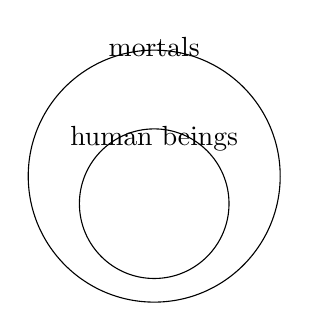
\begin{tikzpicture}[baseline]
  \draw (0,0) circle (1.6cm) node[above=1.4cm] {mortals};
  \draw (0,-0.35) circle (0.95cm) node[above=0.55cm] {human beings};
\end{tikzpicture}
&
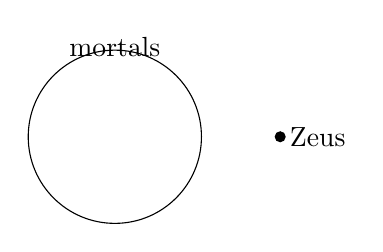
\begin{tikzpicture}[baseline]
  \draw (0,0) circle (1.1cm) node[above=0.9cm] {mortals};
  \fill (2.1,0) circle (2pt) node[right] {Zeus};
\end{tikzpicture}
\end{tabular}
\end{center}

There is only one way to overlay these two pictures consistently:
Zeus's dot must fall outside the human-beings disk too, since that
disk is entirely contained inside the mortals disk he is already
outside of. The conclusion is forced — no admissible way of drawing
the diagrams makes the premises true and the conclusion false.

\begin{experiment}{The syllogism formalized}
\begin{lean}
theorem zeus_syllogism {alpha : Type} (mortal human : alpha → Prop)
    (zeus : alpha)
    (major : ∀ x, human x → mortal x)
    (minor : ¬ mortal zeus) :
    ¬ human zeus := by
  intro hz
  exact minor (major zeus hz)
\end{lean}
The Lean proof is exactly the diagram's reasoning stated
symbolically: \texttt{major zeus hz} produces a proof that Zeus is
mortal from the assumption that he is human, which \texttt{minor}
directly contradicts.
\end{experiment}

\subsection{An Invalid Syllogism, and the Converse Error}

Now change the minor premise: all human beings are mortal; Felix is
mortal; therefore Felix is a human being. The major premise diagram
is unchanged, but the minor premise only says Felix's dot lies
\emph{somewhere} inside the mortals disk — nothing pins it down
relative to the human-beings disk nested inside.

\begin{center}
\begin{tabular}{cc}
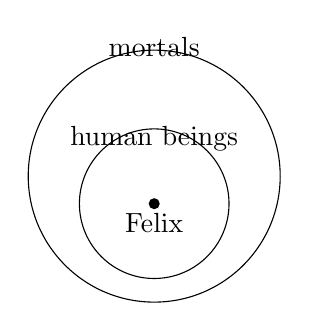
\begin{tikzpicture}[baseline]
  \draw (0,0) circle (1.6cm) node[above=1.4cm] {mortals};
  \draw (0,-0.35) circle (0.95cm) node[above=0.55cm] {human beings};
  \fill (0,-0.35) circle (2pt) node[below] {Felix};
\end{tikzpicture}
&
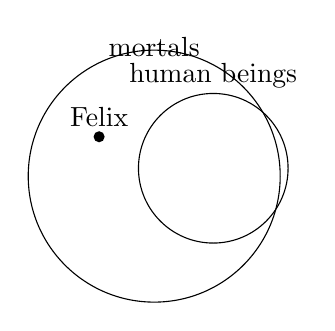
\begin{tikzpicture}[baseline]
  \draw (0,0) circle (1.6cm) node[above=1.4cm] {mortals};
  \draw (0.75,0.1) circle (0.95cm) node[above=0.9cm] {human beings};
  \fill (-0.7,0.5) circle (2pt) node[above] {Felix};
\end{tikzpicture}
\end{tabular}
\end{center}

Both pictures satisfy both premises, and they disagree about the
conclusion: in the first, Felix is a human being; in the second, he
is a mortal non-human — a cat, say. Because the premises do not force
a unique picture, the argument is invalid.

\begin{fallacy}{Converse error}
This argument would be valid if the major premise were replaced by
its converse (``all mortals are human beings''), but a universal
conditional is not logically equivalent to its converse, so no such
replacement is available.
\[
\begin{array}{ll}
\textbf{Formal} & \textbf{Informal} \\[2pt]
\forall x,\ P(x) \to Q(x). & \text{If $x$ makes $P(x)$ true, then $x$ makes $Q(x)$ true.} \\
Q(a),\text{ for a particular } a. & a \text{ makes } Q(x) \text{ true.} \\
\therefore P(a). \quad \leftarrow \text{invalid} & \therefore a \text{ makes } P(x) \text{ true.} \quad \leftarrow \text{invalid}
\end{array}
\]
\end{fallacy}

\begin{fallacy}{Inverse error}
A closely related pattern: this would be valid if a conditional were
logically equivalent to its \emph{inverse}, but it is not.
\[
\begin{array}{ll}
\textbf{Formal} & \textbf{Informal} \\[2pt]
\forall x,\ P(x) \to Q(x). & \text{If $x$ makes $P(x)$ true, then $x$ makes $Q(x)$ true.} \\
\lnot P(a),\text{ for a particular } a. & a \text{ does not make } P(x) \text{ true.} \\
\therefore \lnot Q(a). \quad \leftarrow \text{invalid} & \therefore a \text{ does not make } Q(x) \text{ true.} \quad \leftarrow \text{invalid}
\end{array}
\]
\end{fallacy}

\subsection{An Argument with ``No''}

A universal \emph{negative} statement — ``no polynomial functions
have horizontal asymptotes'' — is pictured as two disks that do not
overlap at all, rather than one nested inside the other.

\begin{center}
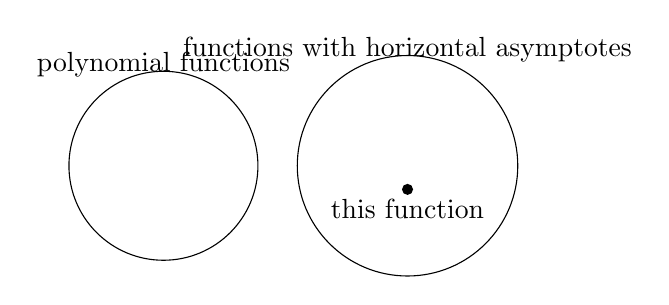
\begin{tikzpicture}
  \draw (0,0) circle (1.2cm) node[above=1cm] {polynomial functions};
  \draw (3.1,0) circle (1.4cm) node[above=1.2cm] {functions with horizontal asymptotes};
  \fill (3.1,-0.3) circle (2pt) node[below] {this function};
\end{tikzpicture}
\end{center}

The argument ``no polynomial functions have horizontal asymptotes;
this function has a horizontal asymptote; therefore this function is
not a polynomial function'' is valid: the dot's disk and the
polynomial-functions disk share no space at all, so the dot cannot
lie in both.

\begin{experiment}{Universal modus tollens}
Transforming ``no $P$ are $Q$'' into ``$\forall x$, if $P(x)$ then
$\lnot Q(x)$'' turns this into an instance of a pattern already
familiar from Chapter~2.
\begin{lean}
theorem no_p_are_q {alpha : Type} (P Q : alpha → Prop) (a : alpha)
    (major : ∀ x, P x → ¬ Q x)
    (minor : Q a) :
    ¬ P a := by
  intro ha
  exact (major a ha) minor
\end{lean}
\end{experiment}

\begin{sidebar}{Disks and ontologies}
The disk-in-disk picture used throughout this section — a category
represented as a region, membership represented as containment,
individuals represented as dots — is not unique to syllogistic logic.
Ontology frameworks such as BFO (Basic Formal Ontology) and the OBO
Foundry organize is-a hierarchies the same way: a subsuming category
contains its subcategories, and reasoning about class membership
reduces to the same containment question these Euler diagrams are
built to answer. The notation differs, but the underlying structure
— subsumption as containment — is the same object viewed twice.
\end{sidebar}

\section{Exercises}

\begin{exercise}
State and prove De Morgan's laws for quantifiers:
$\lnot \forall x, P\,x \leftrightarrow \exists x, \lnot P\,x$
(classically) and identify which direction survives constructively.
\end{exercise}

\begin{exercise}
Draw the Euler diagrams for, and construct an explicit countermodel
to, the inverse-error argument form given above.
\end{exercise}

